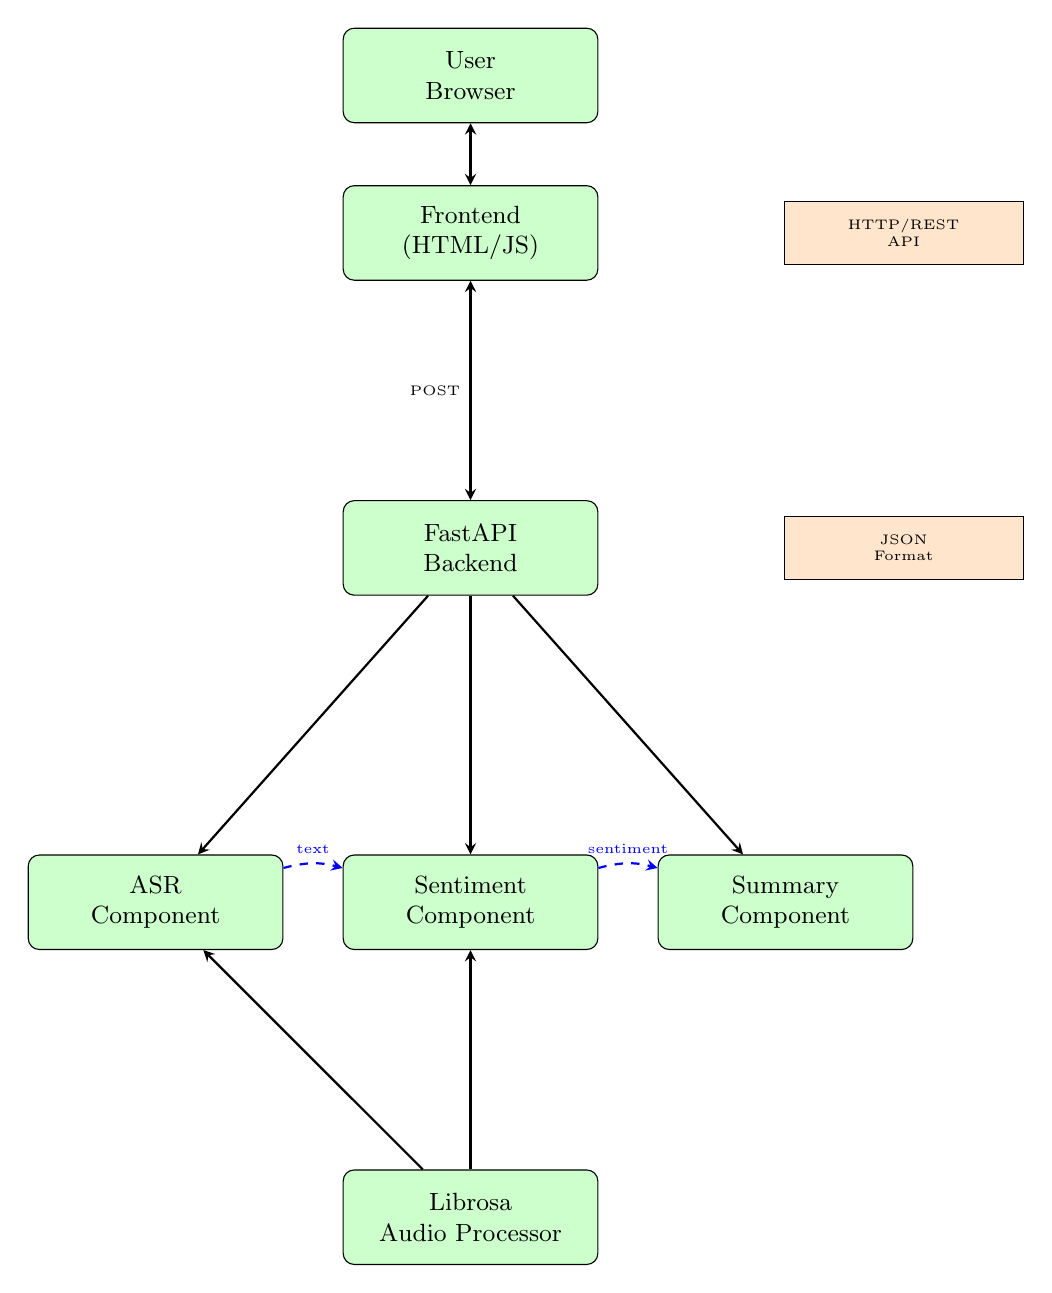
\begin{tikzpicture}[
    node distance=3cm,
    component/.style={rectangle, draw, fill=green!20, text width=3cm, text centered, rounded corners, minimum height=1.2cm, font=\small},
    interface/.style={rectangle, draw, fill=orange!20, text width=2.8cm, text centered, minimum height=0.8cm, font=\tiny},
    arrow/.style={->, >=stealth, thick},
    bidirectional/.style={<->, >=stealth, thick}
]

% Components arranged vertically
\node[component] (frontend) {Frontend\\(HTML/JS)};
\node[component, below of=frontend, yshift=-1cm] (fastapi) {FastAPI\\Backend};

% Three components in a row
\node[component, below of=fastapi, yshift=-1.5cm, xshift=-4cm] (asr_comp) {ASR\\Component};
\node[component, below of=fastapi, yshift=-1.5cm, xshift=0cm] (sentiment_comp) {Sentiment\\Component};
\node[component, below of=fastapi, yshift=-1.5cm, xshift=4cm] (summary_comp) {Summary\\Component};

\node[component, below of=sentiment_comp, yshift=-1cm] (librosa) {Librosa\\Audio Processor};

% Interfaces
\node[interface, right of=frontend, xshift=2.5cm] (http) {HTTP/REST\\API};
\node[interface, right of=fastapi, xshift=2.5cm] (json) {JSON\\Format};

% Arrows
\draw[bidirectional] (frontend) -- node[left, font=\tiny] {POST} (fastapi);
\draw[arrow] (fastapi) -- (asr_comp);
\draw[arrow] (fastapi) -- (sentiment_comp);
\draw[arrow] (fastapi) -- (summary_comp);
\draw[arrow] (librosa) -- (asr_comp);
\draw[arrow] (librosa) -- (sentiment_comp);

% Data flow annotations
\draw[arrow, blue, dashed, thick] (asr_comp) to[bend left=15] node[above, sloped, font=\tiny] {text} (sentiment_comp);
\draw[arrow, blue, dashed, thick] (sentiment_comp) to[bend left=15] node[above, sloped, font=\tiny] {sentiment} (summary_comp);

% External connections
\node[component, above of=frontend, yshift=-1cm] (user) {User\\Browser};
\draw[bidirectional] (user) -- (frontend);

\end{tikzpicture}
